\documentclass{article}

\usepackage[left=2cm,right=2cm, top=2cm, bottom = 2cm]{geometry}
\usepackage{amsfonts}
%%%\usepackage{array}

\usepackage{amsmath}
\usepackage{xcolor}

\usepackage{tikz}
\usepackage{subfigure}

\pagestyle{empty}

\setlength{\tabcolsep}{15pt}
%%%\renewcommand{\arraystretch}{2.5}

%%%\makeatletter
%%%\newcommand{\thickhline}{%
%%%    \noalign {\ifnum 0=`}\fi \hrule height 2pt
%%%    \futurelet \reserved@a \@xhline
%%%}
%%%\newcolumntype{!}{@{\hskip\tabcolsep\vrule width 2pt\hskip\tabcolsep}}
%%%\makeatother

\newcommand{\deriv}[3][]{\frac{\mathrm{d}^{#1} #2}{\mathrm{d}#3^{#1}}}
\newcommand{\cis}{\,\mathrm{cis}}




\begin{document}

\title{Limits to Infinity and Taylor Series}
\date{}

\maketitle
\thispagestyle{empty}

\Large

\textbf{\underline{Objective: To understand the notion of a limit as a variable tends}}

\textbf{\underline{``to infinity,'' and to apply this to Taylor series.}}




\vspace{5mm}


\textbf{Recap: Taylor Polynomials:}

\vspace{5mm}


Let $f(x)=(1+x)^{-1/2}$.
% f'(x) = (-1/2)(1+x)^{-3/2}; f''(x)=(3/4)(1+x)^{-5/2}; f'''(x)=(-15/8)(1+x)^{-7/2}. (15*7/16)(1+x)^{-9/2}

\begin{enumerate}
	\item Compute the degree 3 Taylor polynomial of $f(x)$ about $x=0$. % 1 - 1/2 x + 3/8 x^2 - 5/16 x^3
	\item Estimate the value of $\frac{1}{\sqrt{2}}$ by evaluating your Taylor polynomial at $x=1$.
	\item Show that $\frac{5}{7}\times\left(1+\frac{1}{49}\right)^{-1/2}=\frac{1}{\sqrt{2}}$.
	\item By evaluating your Taylor polynomial at $x=\frac{1}{49}$, obtain an estimate for $\left(1+\frac{1}{49}\right)^{-1/2}$. Hence obtain a second estimate of $\frac{1}{\sqrt{2}}$.
	\item Which of your two estimates is better? Can you explain this?
	\item \textbf{Harder:} Explain how you could accurately approximate $\frac{1}{\sqrt{11}}$? Hint: can you find $x=\frac{c}{b^2}$ such that $1+x=\frac{11\times a^2}{b^2}$ for some integers $a$, $b$, and $c$? % x=10 is a terrible idea. we want \sqrt{1+x}=a\sqrt{11}/b, so 1+x=11a^2/b^2; if x=c/b^2, then b^2+c=11a^2. If a=3, 11a^2=99, so take c=-1, b=10; so x=-1/100. Then 1+x=1-1/100=99/100=9*11/100, so \sqrt{1+x}=3\sqrt{11}/100, so (3/100)(1+x)^{-1/2}=1/\sqrt{11}
\end{enumerate}

\bigskip










\clearpage



\textbf{Theory: Limits to Infinity:}

\vspace{5mm}

We have seen the notion of a limit:
\[\lim_{x\to a}f(x)=L\]
if $f(x)$ gets arbitrarily close to $L$ as $x$ gets close to $a$; more precisely, if for any target zone around $L$, no matter how small, we can find a launch zone around $a$ such that if $x$ is in the launch zone, then $f(x)$ will be in the target zone.

Sometimes, rather than taking $x$ closer and closer to some fixed value $a$, we want to study $f(x)$ as $x$ gets very big; for instance, we may want to study the eventual behaviour of a system after a long time. To do this, we extend our definition of a limit to define the limit of $f(x)$ as $x$ \textbf{tends to infinity}. The idea is essentially the same, but our ``launch zone'' will no longer be a small interval around $a$, but instead consist of large numbers. We define
\[\lim_{x\to \infty}f(x)=L\]
if for any target zone around $L$ there is a number $M$ (think of $M$ as very big) such that if $x$ is in the launch zone of numbers bigger than $M$, then $f(x)$ is in the target zone. More formally:
for any $\epsilon>0$ there exists some $M$ such that if $x>M$, then $L-\epsilon<f(x)<L+\epsilon$.

We can then also define
\[\lim_{x\to -\infty}f(x)=L\]
if for any target zone around $L$ there is a number $M$ (think of $M$ as big but negative) such that if $x$ is in the launch zone of numbers \textit{smaller} than $M$, then $f(x)$ is in the target zone:
for any $\epsilon>0$ there exists some $M$ such that if $x<M$, then $L-\epsilon<f(x)<L+\epsilon$.\bigskip


Find the limit of $\frac{1}{x}$ as $x\to \infty$.

\vfill


Find the limit of $x\sin\left(\frac{1}{x}\right)$ as $x\to \infty$.

\vfill



\clearpage






\textbf{Theory: Infinite Series:}

\vspace{5mm}


When taking the limit of a function as $x$ tends to some value $a$, $x$ needs to be able to take values continuously (\textit{e.g.}, any real value). If $x$ can only take integer values, then once our launch zone around $a$ is small enough, there are no integers in the launch zone (except perhaps $a$ itself, but that is excluded as a value of $x$ when taking the limit), so we cannot proceed.

However, with limits as $x$ tends to infinity, we have no such constraint. No matter how large $M$ is, there will always be integers bigger than $M$, so we can consider integer values of $x$ inside our launch zone. One application of this is that it allows us to consider ``infinite sums,'' typically called \textbf{infinite series}. For instance, to add together the infinite series $1+\frac{1}{2}+\frac{1}{4}+\frac{1}{8}+\frac{1}{16}+\hdots$ (where the $n^{\mathrm{th}}$ term is $2^{-n}$), we can define
\[f(n)=\sum_{i=0}^n 2^{-i}.\]
So $f(0)=1$, $f(1)=1+\frac{1}{2}=\frac{3}{2}$, $f(2)=1+\frac{1}{2}+\frac{1}{4}=\frac{7}{4}$, etc. Then to take the infinite sum, we define
\[\sum_{i=0}^\infty 2^{-i}=\lim_{n\to\infty}f(n)=\lim_{n\to\infty}\sum_{i=0}^n2^{-i}.\]

This looks complicated and intimidating, but really all it's saying is that to add infinitely many numbers together, we add together the first $n$, and see what happens as $n$ gets larger and larger---in other words, we just add our numbers together one at a time and see what value we tend towards.\bigskip

Evaluate $\sum\limits_{i=0}^\infty 2^{-i}$.


\vfill


Evaluate $\sum\limits_{i=0}^\infty r^i$, where $0<r<1$.

\vfill

\clearpage







\textbf{Theory: Convergence and Divergence, Cautions:}

\vspace{5mm}



Be warned: infinite series do not always have a value. An obvious example is
\[\sum_{i=1}^\infty i=1+2+3+4+\hdots\]
Clearly this should be infinity, and indeed we can see that no matter what value $L$ we take as a potential limit, and what $\epsilon$ we take for our target zone, if we choose $M$ big enough, then the sum of the first $M$ terms will be bigger than $L+\epsilon$, so outside the target zone. So no matter what $L$ and $\epsilon$ we pick, we cannot find a launch zone, so the limit cannot exist. In cases like this, we say the infinite series \textbf{diverges}; when the limit does exist, we say the series \textbf{converges}.\bigskip

Show that $\sum\limits_{n=1}^\infty \frac{1}{n}$ diverges.

\vfill


{\color{red}


\textbf{Warning:} There are certain YouTube videos and other sources which claim that it is possible to take the sum of a divergent series; for instance, they claim that the sum of the positive integers at the top of the page is equal to $-\frac{1}{12}$. While there is some real maths behind this, it is much more complicated than popular accounts tends to suggest, involving something called ``the analytic continuation of Riemann's zeta function.'' For almost all purposes, the idea of infinite summation as presented here is the appropriate one to use, and there is no meaningful value for something like the sum of all positie integers; all we can say is that the series diverges.




\clearpage




\textbf{Theory: Absolute and Conditional Convergence:}

\vspace{5mm}



\textbf{Second warning:} The issue of convergence versus divergence is slightly more subtle than presented above. A series 
\[\sum_{n=0}^\infty a_n\]
\textbf{converges absolutely} if
\[\sum_{n=0}^\infty |a_n|\]
converges. If the original series converges, but the series with the modulus in does not, then we say the original series \textbf{converges conditionally}. If neither holds, then the series diverges.

Roughly speaking, absolutely convergent series can be manipulated just like finite sums; you can reorder the terms, group terms together, etc. With conditionally convergent series, however, you have to be very careful, as very strange things can happen if you aren't careful. In particular, Riemann's Summation Theorem says that you can reorder the terms in a conditionally convergent series to change the sum to be anything you like!

It would take a lot of work to cover the theory needed to give more details on this, so the key thing to take away is that if a series is divergent or only conditionally convergent, you should treat it with caution, but if it is absolutely convergent, then it's tame and friendly and behaves much like a finite sum.\bigskip

\bigskip



Show that $\sum\limits_{n=1}^\infty \frac{(-1)^{n+1}}{n}$ converges conditionally, by considering the sum of the first $2k$ terms and the sum of the first $2k+1$ terms.

\vfill
}


\clearpage













\textbf{Theory/Practice: Taylor Series:}


We have seen the Taylor polynomials of a function $f(x)$ around a point $x=a$. The more terms we take (the higher the degree of the polynomial), the more accurately it tends to approximate $f(x)$. Now that we have a notion of infinite sum, we can extend this to define the \textbf{Taylor series} of $f(x)$ about $x=a$ by taking infinitely many terms:
\[f(x)=\sum_{n=0}^\infty \frac{f^{(n)}(a)}{n!}(x-a)^n.\]

Rewriting in terms of $a+h$;
\[f(a+h)=\sum_{n=0}^\infty \frac{f^{(n)}(a)}{n!}h^n.\]

The Taylor series of a function is sometimes also called the \textbf{Taylor expansion} or \textbf{power series} of the function. A Taylor polynomial of degree $n$ is often simply described as ``the terms up to degree $n$ in the Taylor series.''


\begin{enumerate}
	\item Let $f(x)=e^x$.
		\begin{enumerate}
			\item Compute the first 4 terms of the Taylor series of $f(x)$ about $x=0$.
			\item Write down the $n^\mathrm{th}$ term of the Taylor series of $f(x)$ about $0$ and hence the complete Taylor series.
			\item Substitute $x=j\theta$ into your Taylor series to obtain an infinite series expression for $e^{j\theta}$.
		\end{enumerate}
	\item Compute the first 3 non-zero terms of the Taylor series of $f(x)=\log_e(x)$ about $x=1$. Write in the form $\log_e(1+x)=\hdots$.
	\item Given the following Taylor series:
		\begin{align*}
		\sin(\theta)&=\sum_{n=0}^\infty \frac{(-1)^{n}\theta^{2n+1}}{(2n+1)!}\\
		&=\theta-\frac{\theta^3}{3!}+\frac{\theta^5}{5!}-\frac{\theta^7}{7!}+\hdots,\\
		\cos(\theta)&=\sum_{n=0}^\infty \frac{(-1)^n\theta^{2n}}{(2n)!}\\
		&= 1-\frac{\theta^2}{2!}+\frac{\theta^4}{4!}-\frac{\theta^6}{6!}+\hdots
		\end{align*}
		write down the function $\cis(\theta)=\cos(\theta)+j\sin(\theta)$ as an infinite series. Compare with your answer to question 1(c).
\end{enumerate}







\clearpage







\textbf{Theory: Exponentials, Trigonometry, and Complex Numbers:}

\vspace{5mm}


On the last page, we saw an interesting use of Taylor series. An expression like $e^{j\theta}$ does not \textit{a priori} make sense; however, we can input a complex number into a polynomial or a power series just fine, so we can \textit{define} $e^z$, for $z\in\mathbb{C}$, to be the complex number given by the limit of the series:
\[e^z=\sum_{n=0}^\infty \frac{z^n}{n!}\]
for any $z\in \mathbb{C}$. Similarly, we can use Taylor expansions to define the sine, cosine, etc. of complex numbers. So any function we can define on the reals (so long as it is nice enough to have a well-behaved Taylor series) can be extended to complex numbers.

This idea of extending functions to take complex inputs by using their Taylor series also showed us something very interesting in the last question on the previous page. We showed that
\[e^{j\theta}=\cos(\theta)+j\sin(\theta).\]

This is known as \textbf{Euler's Equation}, and is widely considered to be one of the most beautiful and profound results in all of mathematics. In particular, if we take $\theta=\pi$, we get
\[e^{j\pi}=-1,\]
a very surprising relationship between the two irrational numbers $e$ and $\pi$!

Note that $\theta$ in Euler's equation need not be a real angle. Euler's equation holds for any $\theta\in\mathbb{C}$.\bigskip



We have seen that any complex number $z=a+bj$ can be written in \textbf{polar form} as $r\cis(\theta)=r\left(\cos(\theta)+j\sin(\theta)\right)$, where $r=|z|$ is the modulus and $\theta=\arg(z)$ is the argument. Given Euler's equation, we can rewrite this as
\[z=re^{j\theta}.\]

This is sometimes called the \textbf{exponential form} of a complex number; however, since it is still just a way of expressing the modulus and argument, it is also sometimes called the polar form, just like $r\cis(\theta)$---since Euler's equation gives $\cis(\theta)=e^{j\theta}$, the exponential and polar forms of a complex number really are two slightly different ways of writing exactly the same thing!






\clearpage




\textbf{Theory: Radius of Convergence:}

\vspace{5mm}


We have seen that an infinite series can converge or diverge. For a power series, there is a variable in the series, so its convergence will depend on the value of the variable. For instance, the Taylor expansion of $\log_e(x)$ about $x=1$ is
\[\log_e(1+x)=\sum_{n=1}^\infty \frac{(-1)^{n+1}x^n}{n}.\]
When $x=\frac{1}{2}$, this is
\[\sum_{n=1}^\infty \frac{(-1)^{n+1}}{n2^n}=\frac{1}{2}-\frac{1}{8}+\frac{1}{24}-\frac{1}{64}+...,\]
which converges; this can be seen by a similar method to how we showed that $\sum\frac{(-1)^n}{n}$ converges, by considering the sum of the first $2k$ terms and the sum of the first $(2k+1)$ terms. So for $x=\frac{1}{2}$, we can use the Taylor series to find $\log_e\left(\frac{3}{2}\right)$. On the other hand, if we take $x=-1$, we get
\[\sum_{n=1}^\infty \frac{1}{n}=1+\frac{1}{2}+\frac{1}{3}+\frac{1}{4}+\hdots,\]
which we showed above diverges. This is not surprising, since at $x=-1$ we get $\log_e(0)$, which is undefined---so we wouldn't expect the Taylor series to give a sensible answer!

Given the Taylor expansion of a function $f(x)$ about a point $a$, the \textbf{radius of convergence} is defined to be the shortest distance from $a$ to a point where the series diverges. In other words, if $x$ is closer to $a$ than the radius of convergence, then the Taylor series converges, and if $x$ is further from $a$ than the radius of convergence, the series diverges. For $\log_e(1+x)$, the radius of convergence is 1; so for any $x\in(-1,1)$, we can use the Taylor series to find $\log_e(1+x)$, but for values of $x$ bigger than 1 (or less than $-1$), the Taylor series diverges.

For $e^x$, $\sin(x)$, and $\cos(x)$, the radius of convergence is infinite; \textit{i.e.}, the Taylor series for these functions converge no matter what $x$ is, so we can use the Taylor series without worrying. The general rule is that the radius of convergence is the shortest distance to a point where the original function is undefined. For instance, we saw with $\log_e(1+x)$ above, that for $x=-1$ we get $\log_e(0)$, which is undefined, so the radius of convergence is 1. However, we can Taylor expand $\log_e(x)$ about a different point, say about $50$, and then have a power series for $\log_e(50+x)$ whose radius of convergence will be $50$ (as this is the distance from the centre of the expansion to the closest point where $\log$ is undefined).


\clearpage




\textbf{Practice:}

\vspace{5mm}


\begin{enumerate}
	\item Compute the Taylor series for $(1+x)^{-1}$ about $x=0$. What will its radius of convergence be?
	\item Compute the first 3 terms of the Taylor expansion of $(4x)^{-1/2}$ about $x=7$. What will its radius of convergence be?
	\item \textbf{Harder! Cautionary example:} Let $f(x)=\frac{1}{1+e^x}$.
		\begin{enumerate}
			\item Compute the first 3 non-zero terms of the Taylor series of $f(x)$ about $x=0$. What would you expect the radius of convergence to be?
			\item The graphs of $f(x)$ and its Taylor series are shown below. Based on these graphs, what do you think the radius of convergence is?
			\item By considering $f(j\pi)$, state the radius of convergence.
		\end{enumerate}
\end{enumerate}

\begin{center}
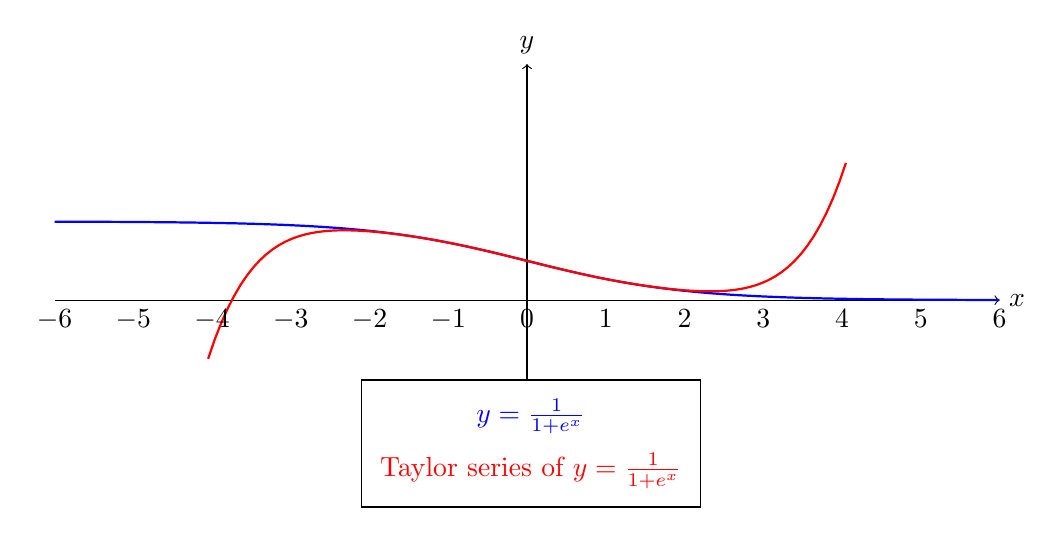
\begin{tikzpicture}
	\draw[->] (-6,0) -- (6,0);
	\node[right] at (6,0) {$x$};
	\draw[->] (0,-1) -- (0,3);
	\node[above] at (0,3) {$y$};
	
	\draw[thick,blue,domain=-6:6,samples=100] plot (\x,{1/(1+2.71828^\x)});
	\draw[thick,red,domain=-4.05:4.05, samples=100] plot (\x, {0.5 - (\x/4) + (\x^3)/48 -(\x^5)/480+(1.7*\x)*(\x^5)*(\x/2)/4032 - (3.1*\x)*(\x/10)*(\x/2)*(\x/2)*(\x/2)*(\x/2)*(\x^3/9072)});
	
	%1/2 - x/4 + x^3/48 - x^5/480 + (17 x^7)/80640 - (31 x^9)/1451520 + (691 x^11)/319334400 + O(x^13)
	
	\foreach \i in {-6,-5,-4,-3,-2,-1,0,1,2,3,4,5,6}{
		\node[below] at (\i,0) {$\i$};
	}
	
	\matrix [draw,below] at (current bounding box.south){
		\node[blue] {$y=\frac{1}{1+e^x}$};\\
		\node[red] {Taylor series of $y=\frac{1}{1+e^x}$};\\
	};
\end{tikzpicture}
\end{center}









\clearpage


{\bf Key Points to Remember:}

\vspace{5mm}

\begin{enumerate}
	\item The limit of a function $f(x)$ as $x$ \textbf{tends to infinity} is $L$ if we can get $f(x)$ as close to $L$ as we like by taking $x$ sufficiently large. This works also for functions with integer inputs.
	\item An \textbf{infinite series} is the sum of infinitely many terms; it is defined by taking the sum of the first $n$ terms, then taking the limit as $n$ tends to infinity:
		\[\sum_{i=0}^\infty a_i=\lim_{n\to\infty}\sum_{i=0}^n a_i,\]
		where the $a_i$ are some numbers.
	\item An infinite series \textbf{converges} if the limit exists (\textit{i.e.}, if it can be summed and give a finite answer); otherwise, the series \textbf{diverges}.
	\item Given an infinitely differentiable function $f(x)$, the \textbf{Taylor series} of $f(x)$ about $x=a$ is the infinite series:
		\[f(x)=\sum_{n=0}^\infty \frac{f^{(n)}(a)}{n!}(x-a)^n,\]
		also written as
		\[f(a+h)=\sum_{n=0}^\infty \frac{f^{(n)}(a)}{n!}h^n.\]
	\item The \textbf{radius of convergence} of the Taylor series of a function $f(x)$ is the distance from $a$ to the closest value of $x$ at which the Taylor series diverges. The Taylor series can only be evaluated for values of $x$ closer to $a$ than the radius of convergence.
	\item The radius of convergence can be found by taking the distance from $a$ to the closest point at which the original function $f(x)$ is undefined---but this could be a complex point, even if we are only interested in real values of the function!
	\item Euler's equation:
		\[e^{jx}=\cos(x)+j\sin(x).\]
	\item The \textbf{exponential form} of a complex number $z$ is $|z|e^{j\arg(z)}$; this is interchangeable with the polar form.
	\item The Taylor expansions for some common functions are given overleaf, with their radii of convergence. For $\log_e(x)$ and $\frac{1}{x}$, the expansion is given about $x=1$, for all others, it is given about $x=0$.
\end{enumerate}

\clearpage

\textbf{Important Taylor Series:}

\vspace{5mm}

\begin{align*}
	e^x&=\sum_{n=0}^\infty \frac{x^n}{n!}\qquad\mbox{ r.o.c.=$\infty$}\\
	&=1+x+\frac{x^2}{2!}+\frac{x^3}{3!}+\hdots\\
	\sin(x)&=\sum_{n=0}^\infty \frac{(-1)^{n}x^{2n+1}}{(2n+1)!}\qquad\mbox{ r.o.c.=$\infty$}\\
	&=x-\frac{x^3}{3!}+\frac{x^5}{5!}-\frac{x^7}{7!}+\hdots,\\
	\cos(x)&=\sum_{n=0}^\infty \frac{(-1)^n x^{2n}}{(2n)!}\qquad\mbox{ r.o.c.=$\infty$}\\
	&= 1-\frac{x^2}{2!}+\frac{x^4}{4!}-\frac{x^6}{6!}+\hdots\\
	\ln(1+x)&=\sum_{n=1}^\infty \frac{(-1)^{n+1}x^n}{n}\qquad\mbox{ r.o.c.=$1$}\\
	&=x-\frac{x^2}{2}+\frac{x^3}{3}-\frac{x^4}{4}+\hdots\\
	(1+x)^{-1}&=\sum_{n=0}^\infty (-x)^n\qquad\mbox{ r.o.c.=$1$}\\
	&= 1 -x+x^2-x^3+\hdots
\end{align*}









\end{document}